\begin{titlepage}
  \backgroundsetup{
  scale=1,
  opacity=1,
  angle=0,
  position=current page.north,
  vshift=-106pt,
  contents={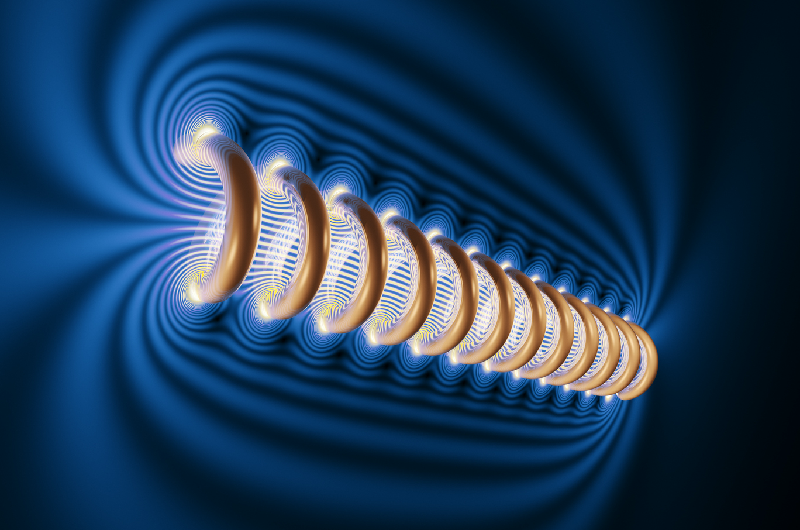
\includegraphics[width=\paperwidth]{FigurasMemoria/imagenPortada.png}}}

  \BgThispage
  \begin{tikzpicture}[remember picture, overlay]
      \fill[maroon] (current page.north west) rectangle ([xshift=2cm]current page.south west);
      \node[rotate=90, anchor=north] at ([xshift=0.6cm, yshift=-10cm]current page.west) {\textcolor{white}{\textbf{\large Pedro José Romero Gombau}}};
      \node[rotate=90, anchor=north] at ([xshift=0.6cm, yshift=2.5cm]current page.west) {\textcolor{white}{\textbf{\large \parbox{13cm}{Diseño y desarrollo de una lanzadera electromagnética}}}};
      \node[rotate=90, anchor=north] at ([xshift=0.6cm, yshift=11cm]current page.west) {\textcolor{white}{\textbf{\large Julio 2024}}};
      \node[anchor=south west, xshift=2.5cm, yshift=0cm] at (current page.south west) {
\includegraphics[width=4.5cm]{FigurasMemoria/logoTecnun.png}};
  \end{tikzpicture}
  \vspace*{10cm}
  
  \begin{flushleft}
      \hspace*{3cm} % Ajusta este valor para mover todo el contenido hacia la derecha
      \begin{minipage}{0.7\textwidth} % Ajusta el ancho de la minipage según sea necesario
          \justifying
          \Huge \textcolor{maroon}{\textbf{Diseño y desarrollo de una lanzadera electromagnética}}
          \vspace*{3.5cm}
          \Large
          \\
          \textcolor{maroon}
          {\textbf{Proyecto Final de Grado}} presentado para obtener el título de Ingeniería Eléctrica por \textcolor{maroon}{\textbf{Pedro José Romero Gombau}} bajo la supervisión de \textcolor{maroon}{\textbf{Ibon Elosegui Simón}}\\\\
          Donostia-San Sebastián, Julio 2024
      \end{minipage}
  \end{flushleft}

\end{titlepage}

\backgroundsetup{contents={}}